\section{Bonos}
\subsection{Uso de Zotero para citación en el documento}
\begin{figure}[H]
\centering
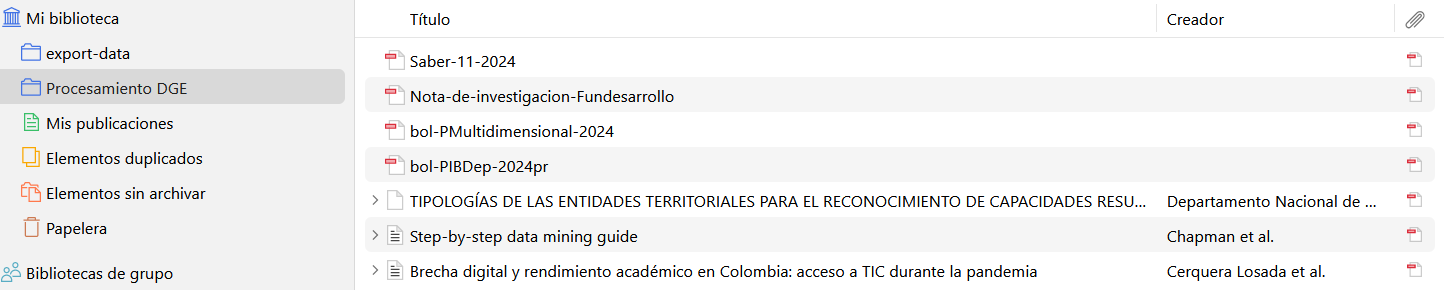
\includegraphics[width=0.9\textwidth]{figures/image2.png}
\caption{Imágen 1. Interfaz de Zotero con las citas}
\end{figure}
\subsection{Web Scrapper}
El dataset de Saber 11 está publicado en datos.gov.co, que usa una plataforma llamada Socrata. Esta plataforma expone los datos directamente como una API REST (llamada SODA), lo que significa que en lugar de parsear HTML de una página web, simplemente hacemos peticiones HTTP a una URL que devuelve los datos en formato JSON. Para no descargar todo de un golpe (el dataset puede tener millones de filas), la función fetch\_all\_rows() usa paginación: pide los datos en bloques de 50.000 registros cambiando el parámetro \$offset en cada petición, hasta obtenerlos todos.
Una vez descargados, los datos se cargan en PySpark para procesarlos de forma distribuida. Spark los convierte en un DataFrame, se limpian las columnas (cast de puntajes a números, estandarización de texto) y se registra una vista SQL para poder hacer consultas directamente. Finalmente, los resultados se convierten a Pandas para graficarlos con matplotlib en 4 visualizaciones: puntajes por departamento, colegios oficiales vs. no oficiales, relación con el estrato socioeconómico, y distribución por período.
Se generaron cuatro gráficas: la primera muestra que Bogotá, Boyacá y Santander lideran en puntaje global promedio (entre 264 y 274 puntos), mientras que Antioquia queda en la parte baja del top 15 con 249; la segunda confirma que los colegios no oficiales superan a los oficiales en las tres áreas evaluadas (global, matemáticas e inglés); la tercera evidencia una relación clara entre nivel socioeconómico y desempeño, donde a mayor estrato mayor puntaje, pasando de 237 en estrato 1 hasta 310 en estrato 6, con la excepción de la categoría “Sin Estrato”, que baja a 212, posiblemente por datos atípicos o población rural; finalmente, la cuarta muestra que el dataset abarca desde 2014 hasta 2021, con 2019 (semestre 4) como el periodo con más estudiantes registrados (alrededor de 90.000), y que los semestres “2” de cada año tienen muchos menos registros que los “1”.
\begin{figure}[H]
\centering
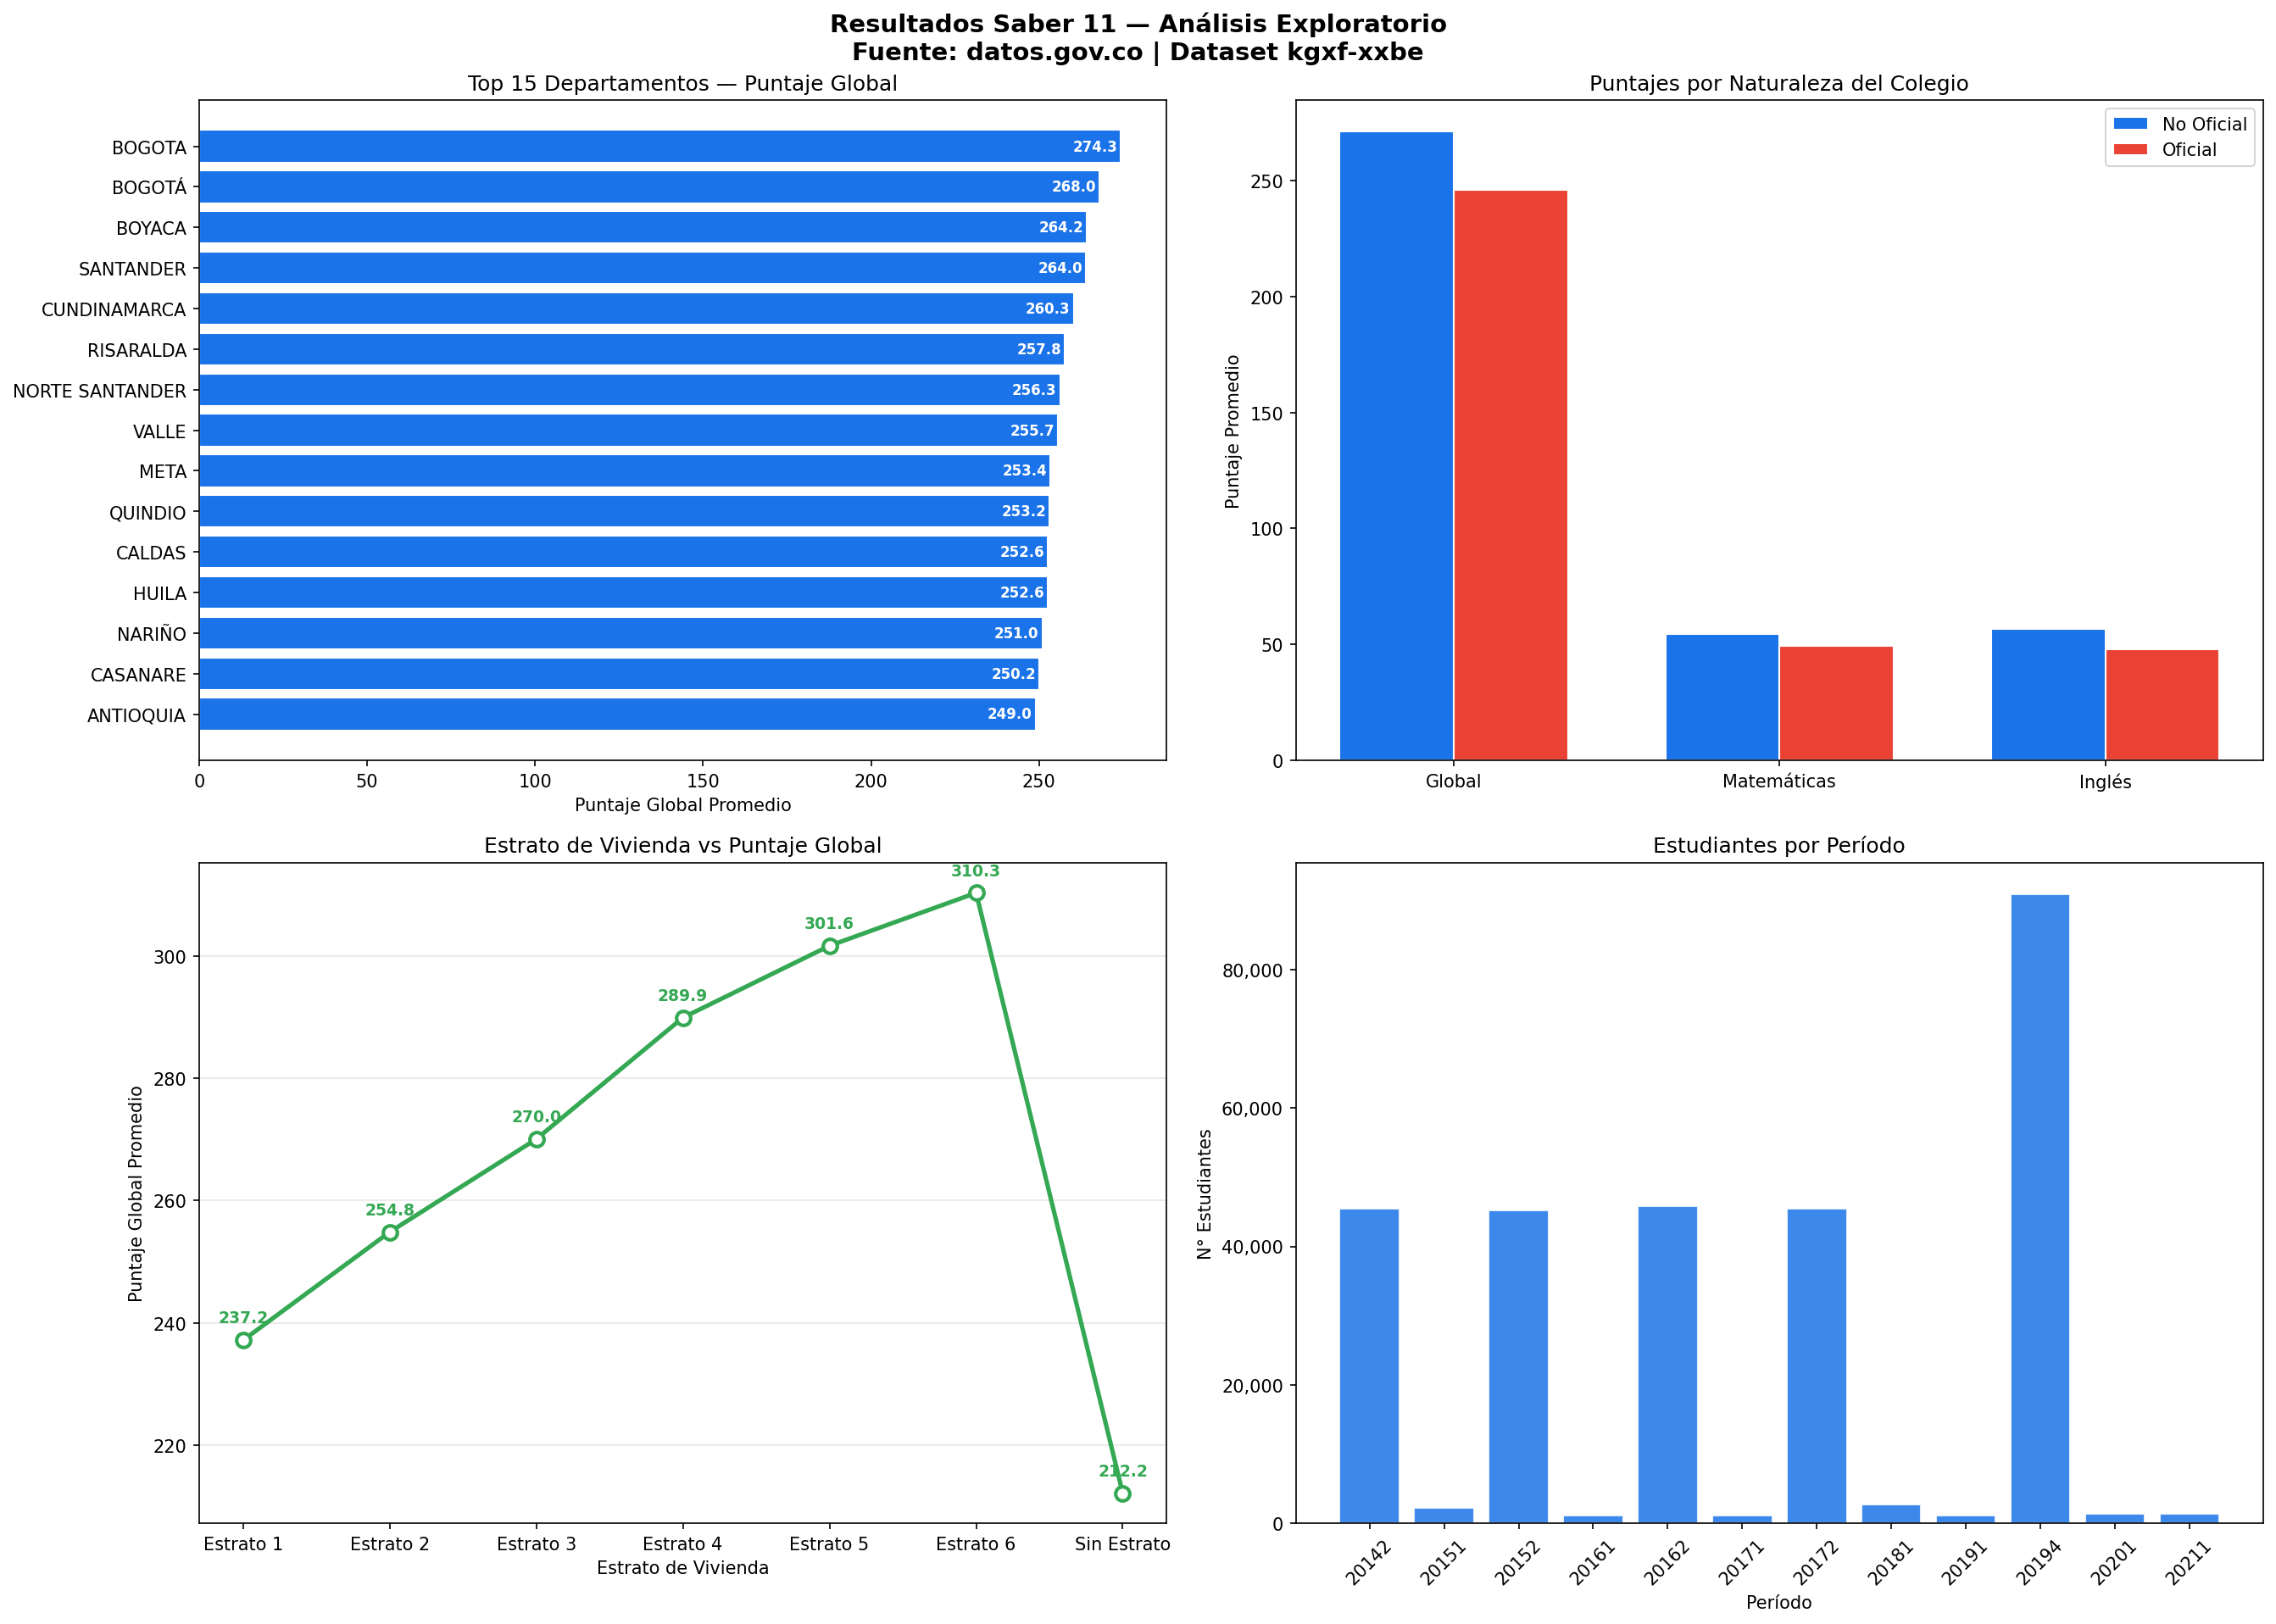
\includegraphics[width=0.9\textwidth]{figures/image3.png}

\caption{Imágen 2. Resultados gráficos saber 11 usando web scrapper}
\end{figure}
\subsection{API del Clima}
La API de OpenWeatherMap expone datos climáticos mediante un endpoint REST gratuito (/data/2.5/forecast) al que se le hace una petición HTTP pasando el nombre de la ciudad y la API key como parámetros. Por cada ciudad, la API devuelve un JSON con 40 bloques de pronóstico (uno cada 3 horas durante 5 días), con información como temperatura, humedad, velocidad del viento y probabilidad de lluvia. La función fetch\_forecast() recorre las 12 ciudades colombianas, aplana cada respuesta JSON en una lista de diccionarios y los junta todos en una sola colección.
Una vez con todos los datos descargados, se cargan en un DataFrame de PySpark con schema explícito para procesarlos de forma distribuida. Se registra una vista SQL para hacer 4 análisis: resumen por ciudad, pronóstico día a día de Bogotá, ranking de ciudades más lluviosas, y variación de temperatura por hora del día. Finalmente los resultados se convierten a Pandas para graficarlos en 4 visualizaciones con matplotlib.
Se generaron cuatro gráficas: la primera muestra que Barranquilla, Cartagena y Cúcuta son las ciudades más cálidas (alrededor de 27°C), mientras que Bogotá y Pasto son las más frías (entre 13 y 14°C), lo cual se explica por la altitud; la segunda evidencia que Pereira, Manizales y Cali tienen la mayor probabilidad de lluvia esta semana (más del 80\%), mientras que Cartagena, Cúcuta y Barranquilla presentan las menores (por debajo del 37\%) a pesar de ser las más calientes; la tercera muestra el pronóstico diario de Bogotá, donde el 11 de abril sería el día más frío (cerca de 12°C) y con mayor probabilidad de lluvia (alrededor del 60\%), y hacia el 13 de abril la temperatura aumenta ligeramente; finalmente, la cuarta gráfica indica que, en promedio, la temperatura sube progresivamente desde las 6 a.m. hasta las 6 p.m. (de unos 19°C a 26°C), mientras que la humedad sigue el comportamiento contrario, bajando al mediodía y recuperándose en la noche.
\begin{figure}[H]
\centering
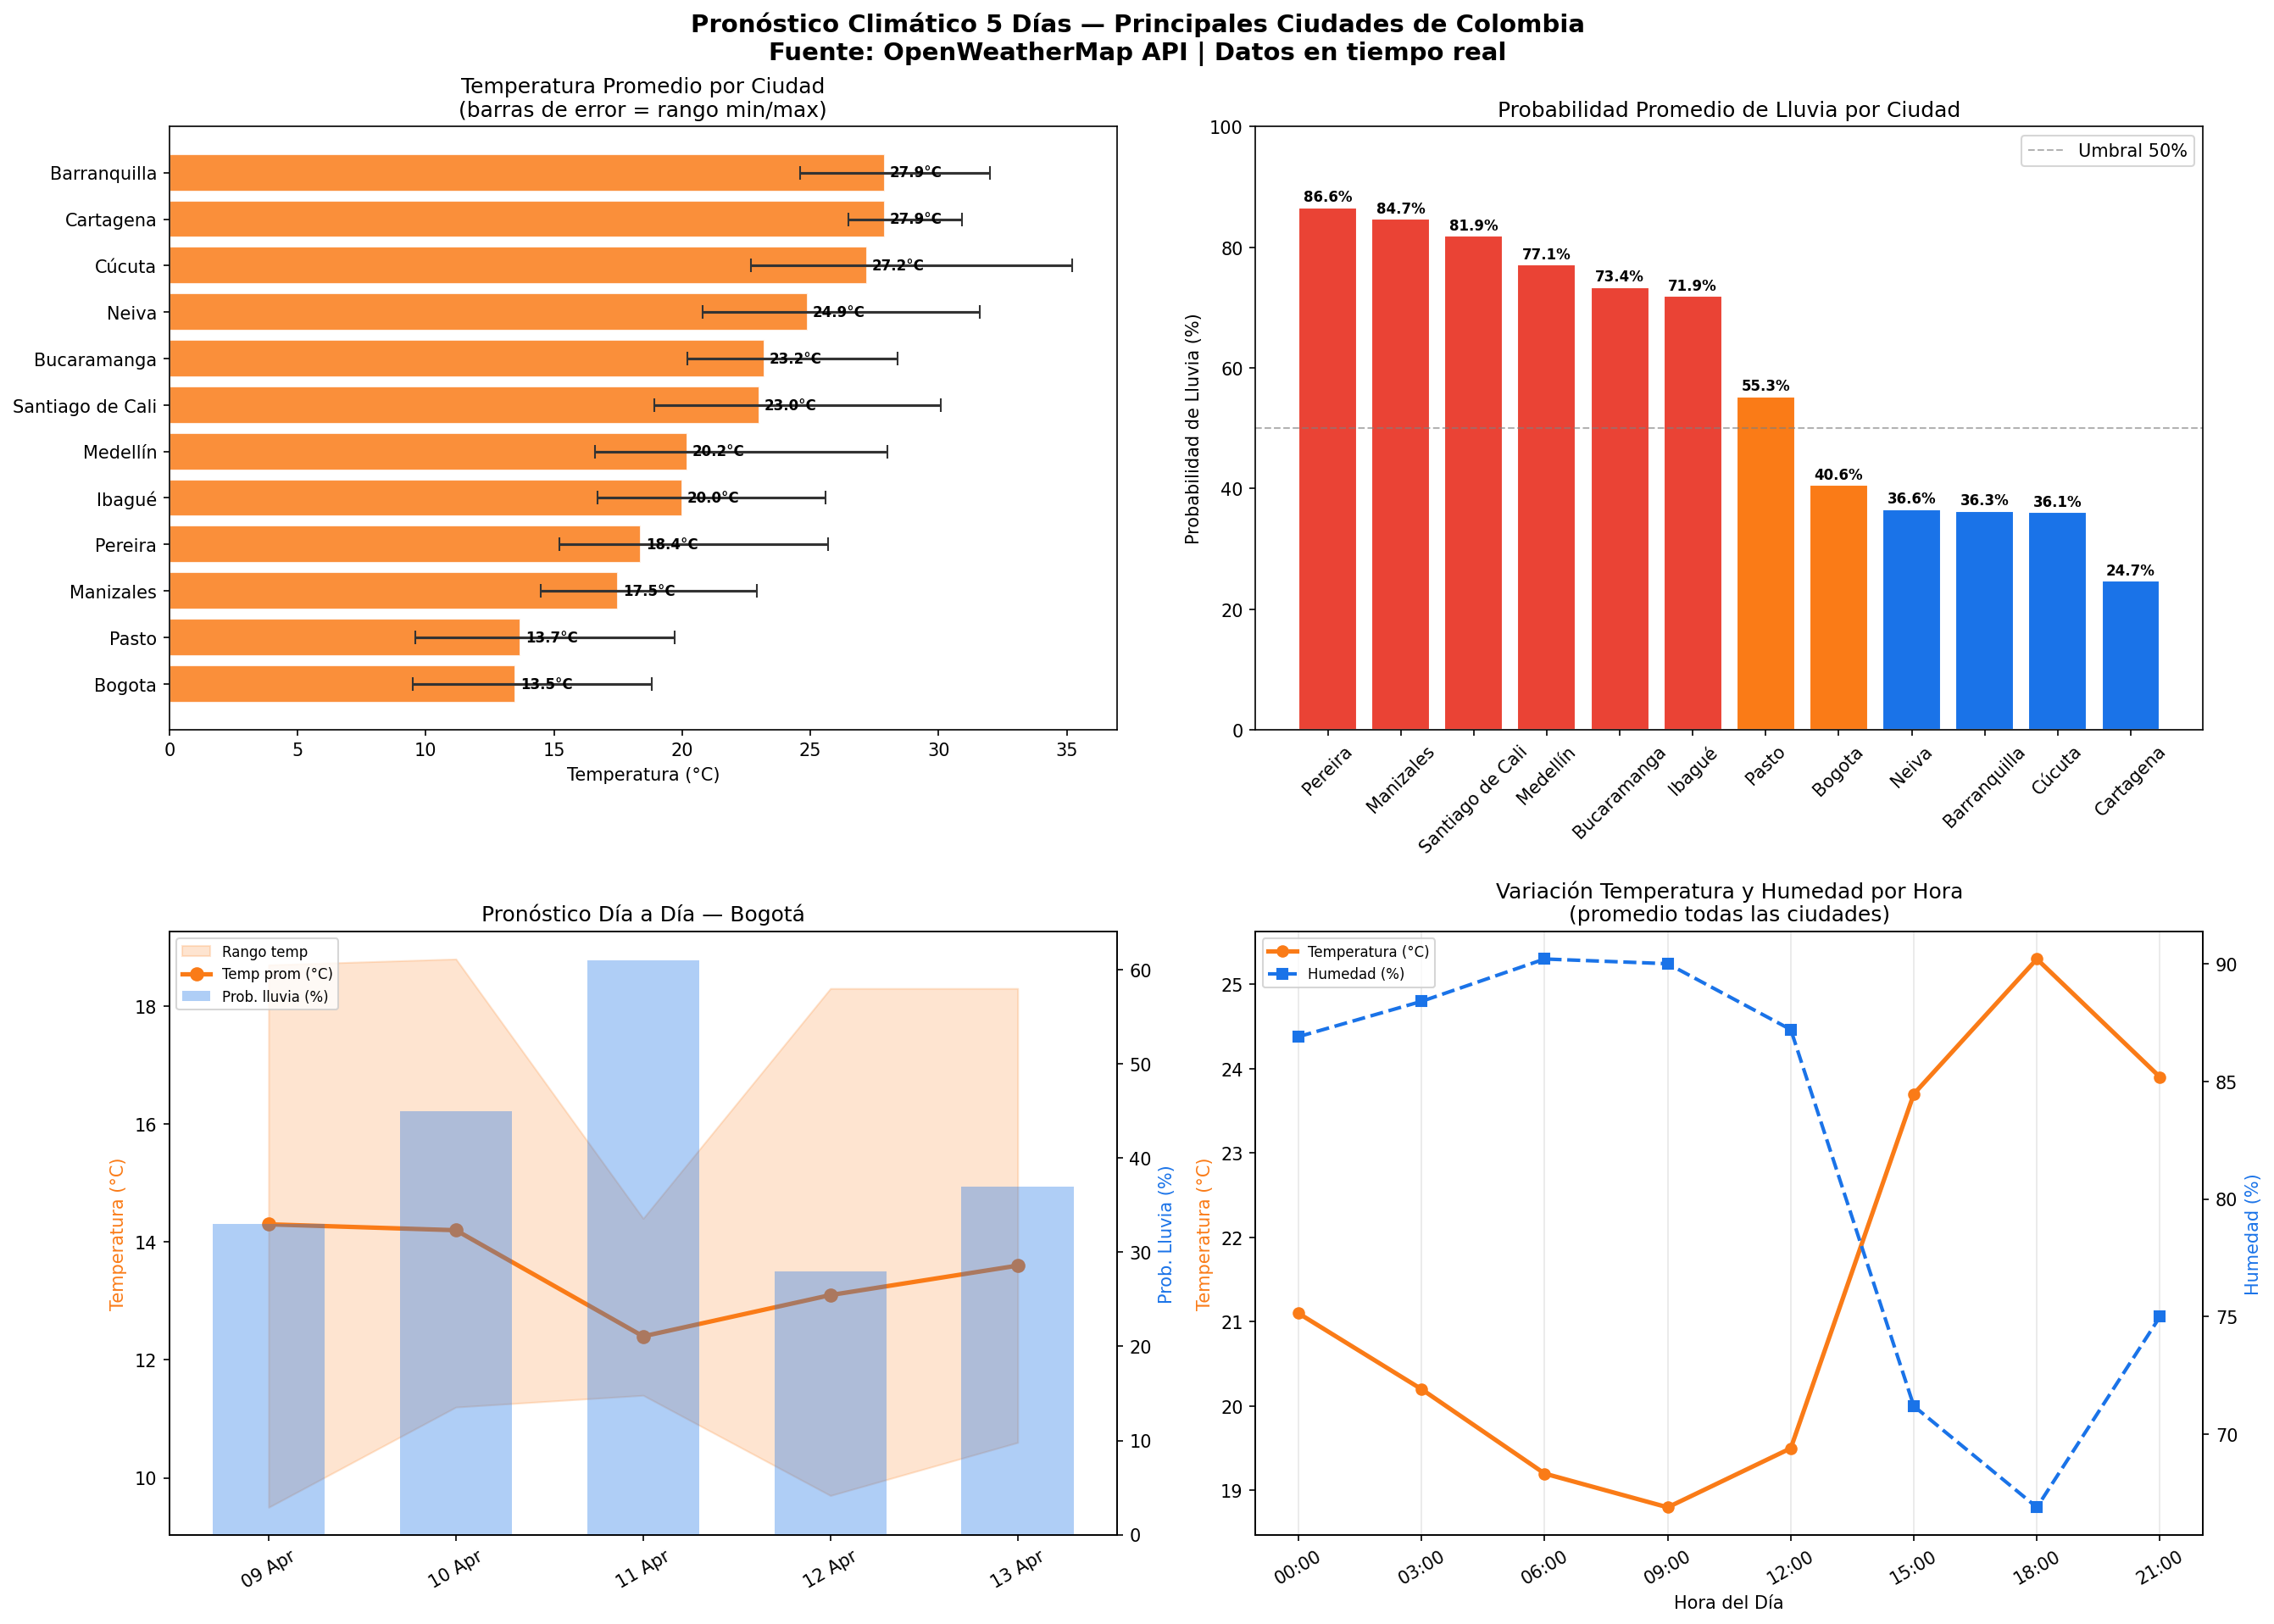
\includegraphics[width=0.9\textwidth]{figures/image4.png}
\caption{Imágen 3. Resultados pronósticos del clima en 5 días}
\end{figure}

\subsection{Modelo de Aprendizaje Profundo (MLP)}
Como bono de la Entrega 2 se construyó un modelo de aprendizaje profundo utilizando el algoritmo \texttt{MultilayerPerceptronClassifier} del paquete \texttt{pyspark.ml.classification}, una red neuronal feed-forward que se entrena distribuidamente sobre el cluster Spark. La elección de este algoritmo responde a tres criterios: se mantiene dentro del ecosistema PySpark MLlib utilizado en el resto del proyecto (evitando dependencias externas como TensorFlow o Keras), se ejecuta sobre los cuatro workers del cluster aprovechando su capacidad de cómputo distribuido, y permite reformular el problema como una clasificación multi-clase a nivel del estudiante individual, lo que complementa los modelos municipales construidos en la sección de resultados.

Mientras que la Regresión Lineal y el Árbol de Decisión predicen el puntaje promedio de un municipio, este modelo predice directamente el \textbf{rango de puntaje} (BAJO, MEDIO o ALTO) de un estudiante individual a partir de su perfil socioeconómico y de colegio. El cambio de unidad de análisis es relevante porque habilita un caso de uso distinto: identificar, antes de que el estudiante presente la prueba, su nivel de riesgo académico, lo que permite al Ministerio focalizar acciones de acompañamiento individualizado.

\textbf{Datos y preparación.} El modelo se entrenó sobre los 4,500,067 registros de estudiantes del Silver ICFES, distribuidos en tres clases: BAJO (699,135 estudiantes, 15.5\%), MEDIO (2,975,241 estudiantes, 66.1\%) y ALTO (825,691 estudiantes, 18.4\%). Las features de entrada son diez variables categóricas (área de ubicación del colegio, naturaleza, jornada, calendario, carácter, género del colegio, género del estudiante, estrato familiar y departamento) más dos binarias (tener internet y tener computador en el hogar). Las categóricas pasaron por \texttt{StringIndexer} y \texttt{OneHotEncoder}, las binarias se mantuvieron numéricas, y todas se ensamblaron en un \texttt{VectorAssembler} seguido de \texttt{StandardScaler}. El pipeline completo de preprocesamiento consta de 23 etapas y produce un vector de entrada de \textbf{76 dimensiones} (después de la codificación one-hot).

\textbf{Pruebas con diferentes arquitecturas.} Para cumplir con el requisito de pruebas con diferentes parámetros, se entrenaron tres arquitecturas distintas sobre una muestra del 10\% del dataset (450,167 estudiantes, 80\% para entrenamiento y 20\% para prueba). El criterio de selección fue el F1-score sobre el conjunto de test, considerando que las clases están desbalanceadas y este indicador es más robusto que la simple exactitud.

\begin{table}[H]
\centering
\caption{Resultados del grid de arquitecturas MLP sobre la muestra del 10\%.}
\begin{tabular}{l r r r r}
\toprule
\textbf{Arquitectura} & \textbf{Parámetros} & \textbf{TEST Acc.} & \textbf{TEST F1} & \textbf{Tiempo (s)} \\
\midrule
$76 \rightarrow 32 \rightarrow 3$              & 2,563 & \textbf{0.6889} & \textbf{0.6315} & 28.2 \\
$76 \rightarrow 64 \rightarrow 3$              & 5,123 & 0.6895 & 0.6302 & 45.6 \\
$76 \rightarrow 64 \rightarrow 32 \rightarrow 3$ & 7,107 & 0.6892 & 0.6312 & 63.1 \\
\bottomrule
\end{tabular}
\end{table}

Las tres arquitecturas obtuvieron desempeños muy similares, con diferencias de F1 inferiores a $0.002$. La red más simple ($76 \rightarrow 32 \rightarrow 3$, con solo 2,563 parámetros entrenables) es la que mejor balance ofrece entre desempeño y tiempo de entrenamiento, lo que sugiere que la frontera de decisión entre clases no requiere una representación profunda y que añadir capas adicionales solo incrementa el costo computacional sin beneficio significativo.

\textbf{Entrenamiento final sobre el dataset completo.} Tras seleccionar la arquitectura ganadora, se re-entrenó el modelo sobre la totalidad del Silver ICFES (3,601,253 estudiantes en train y 898,814 en test) con \texttt{maxIter=80}. El entrenamiento distribuido sobre los cuatro workers tardó 546 segundos (aproximadamente nueve minutos), y los resultados sobre el conjunto de test son los siguientes.

\begin{table}[H]
\centering
\caption{Métricas del modelo MLP final sobre el dataset completo.}
\begin{tabular}{l r r r r}
\toprule
\textbf{Conjunto} & \textbf{Accuracy} & \textbf{Precision} & \textbf{Recall} & \textbf{F1} \\
\midrule
TRAIN (3.6M) & 0.6900 & 0.6713 & 0.6900 & 0.6335 \\
TEST  (898K) & 0.6899 & 0.6715 & 0.6899 & 0.6335 \\
\bottomrule
\end{tabular}
\end{table}

La estabilidad entre las métricas de train y test es una buena señal de generalización: el modelo no está sobreajustado. La exactitud global del 69\% sobre cerca de 900,000 estudiantes de prueba representa un desempeño respetable para una tarea de clasificación multi-clase sobre datos tabulares socioeconómicos.

\textbf{Matriz de confusión y análisis por clase.} Sin embargo, una métrica global como la exactitud puede ser engañosa cuando las clases están desbalanceadas. La matriz de confusión revela el comportamiento real del modelo por clase.

\begin{table}[H]
\centering
\caption{Matriz de confusión del modelo MLP final (test set, 898,814 estudiantes).}
\begin{tabular}{l r r r r}
\toprule
\textbf{Real $\backslash$ Predicho} & \textbf{ALTO} & \textbf{BAJO} & \textbf{MEDIO} & \textbf{Total real} \\
\midrule
ALTO  & 40,657 & 259    & 124,016 & 164,932 \\
BAJO  & 627    & 22,336 & 117,036 & 139,999 \\
MEDIO & 20,957 & 15,867 & 557,059 & 593,883 \\
\bottomrule
\end{tabular}
\end{table}

\begin{table}[H]
\centering
\caption{Precision y recall por clase.}
\begin{tabular}{l r r}
\toprule
\textbf{Clase} & \textbf{Precision} & \textbf{Recall} \\
\midrule
ALTO   & 0.6532 & 0.2465 \\
BAJO   & 0.5807 & 0.1595 \\
MEDIO  & 0.6980 & 0.9380 \\
\bottomrule
\end{tabular}
\end{table}

\begin{figure}[H]
\centering
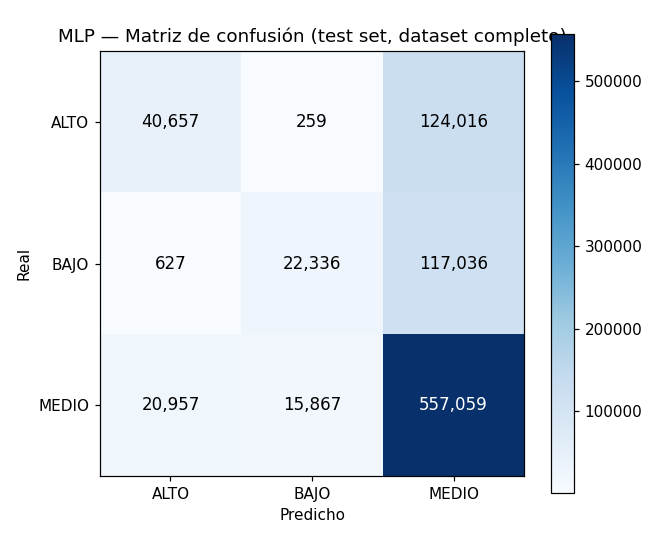
\includegraphics[width=0.7\textwidth]{figures/mlp_confusion_matrix.png}
\caption{Matriz de confusión del modelo MLP final.}
\end{figure}

La interpretación es clara: el modelo es muy preciso identificando estudiantes de la clase mayoritaria MEDIO (recall del 94\%), pero tiene dificultad para identificar correctamente a los estudiantes de las clases minoritarias ALTO (recall 25\%) y BAJO (recall 16\%). Esto se debe al fuerte desbalance del dataset (MEDIO representa el 66\% de los registros), y es un comportamiento esperable cuando no se aplican técnicas específicas de manejo de clases desbalanceadas como sobre-muestreo, ponderación de clases o ajuste de umbrales de decisión.

A pesar de esta limitación, el modelo ofrece valor real como herramienta de \textit{cribado} (filtrado preliminar): permite identificar con alta confianza a los estudiantes con perfil de rendimiento medio, dejando un grupo más pequeño que requiere análisis más detallado para distinguir entre desempeño alto y bajo. La precision de las predicciones positivas (65\% para ALTO, 58\% para BAJO, 70\% para MEDIO) es mejor que el azar y útil como insumo para la priorización de recursos pedagógicos.

\textbf{Persistencia y trabajo futuro.} El modelo final, junto con su pipeline de preprocesamiento, se persistió en HDFS en \texttt{/usr/proyecto/models/mlp\_rango\_estudiante} y \texttt{/usr/proyecto/models/mlp\_rango\_estudiante\_pipeline}, lo que permite cargarlo en cualquier sesión Spark futura para inferir el rango de puntaje de nuevos estudiantes sin tener que repetir el entrenamiento. Una línea natural de trabajo futuro es aplicar técnicas de balanceo de clases (SMOTE, class weights) o cambiar a una formulación binaria (BAJO vs no-BAJO) para construir un sistema de alerta temprana específicamente enfocado en estudiantes en riesgo académico, donde un mayor recall sobre la clase minoritaria es prioritario.